\documentclass[12pt]{article}

\title{Image Analysis Coursework}
\author{James Hughes\\ Word count: 0}

\usepackage{amsfonts}
\usepackage{amsmath}
\usepackage{graphicx}

\begin{document}

\maketitle

\newpage

\tableofcontents

\newpage

\section{Introduction}

\section{Image Segmentation}

\subsection{CT Image}

\begin{figure}[hp]
    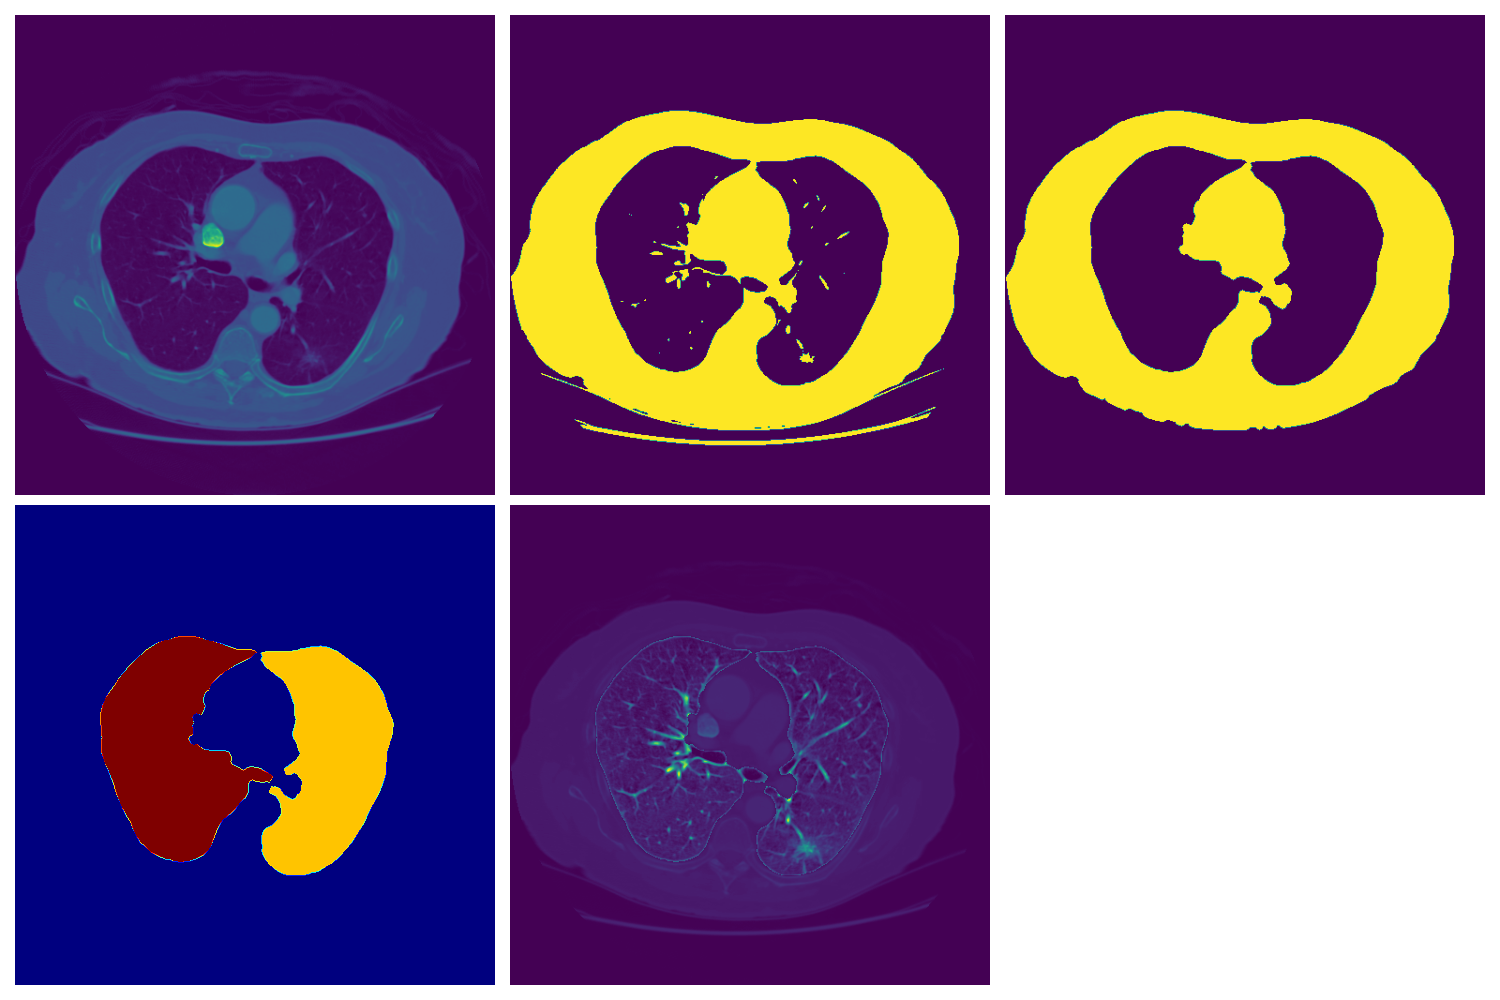
\includegraphics[scale=0.35]{figures/ct_segmentation.png}
    \caption{Steps of CT Segmentation}
    \label{fig:ct}
\end{figure}

The CT scan image was segmented using Otsu's method for image segmentation.
This was an appropriate, simple method which is suited to the monochrome image.
This method easily segments the tissue and bone surrounding the lungs,
distinguishing this from the lugns themselves and the surrounding background.
The segmented image was then post-processed with `binary closing', a morphological operation,
as well as Scikit-Image's \texttt{morphology.remove\_small\_objects} method.
The four segmented regions of the image were then labelled, and the lungs chosen as the smallest masks by area.

\subsection{Flowers Image}

\begin{figure}[hp]
    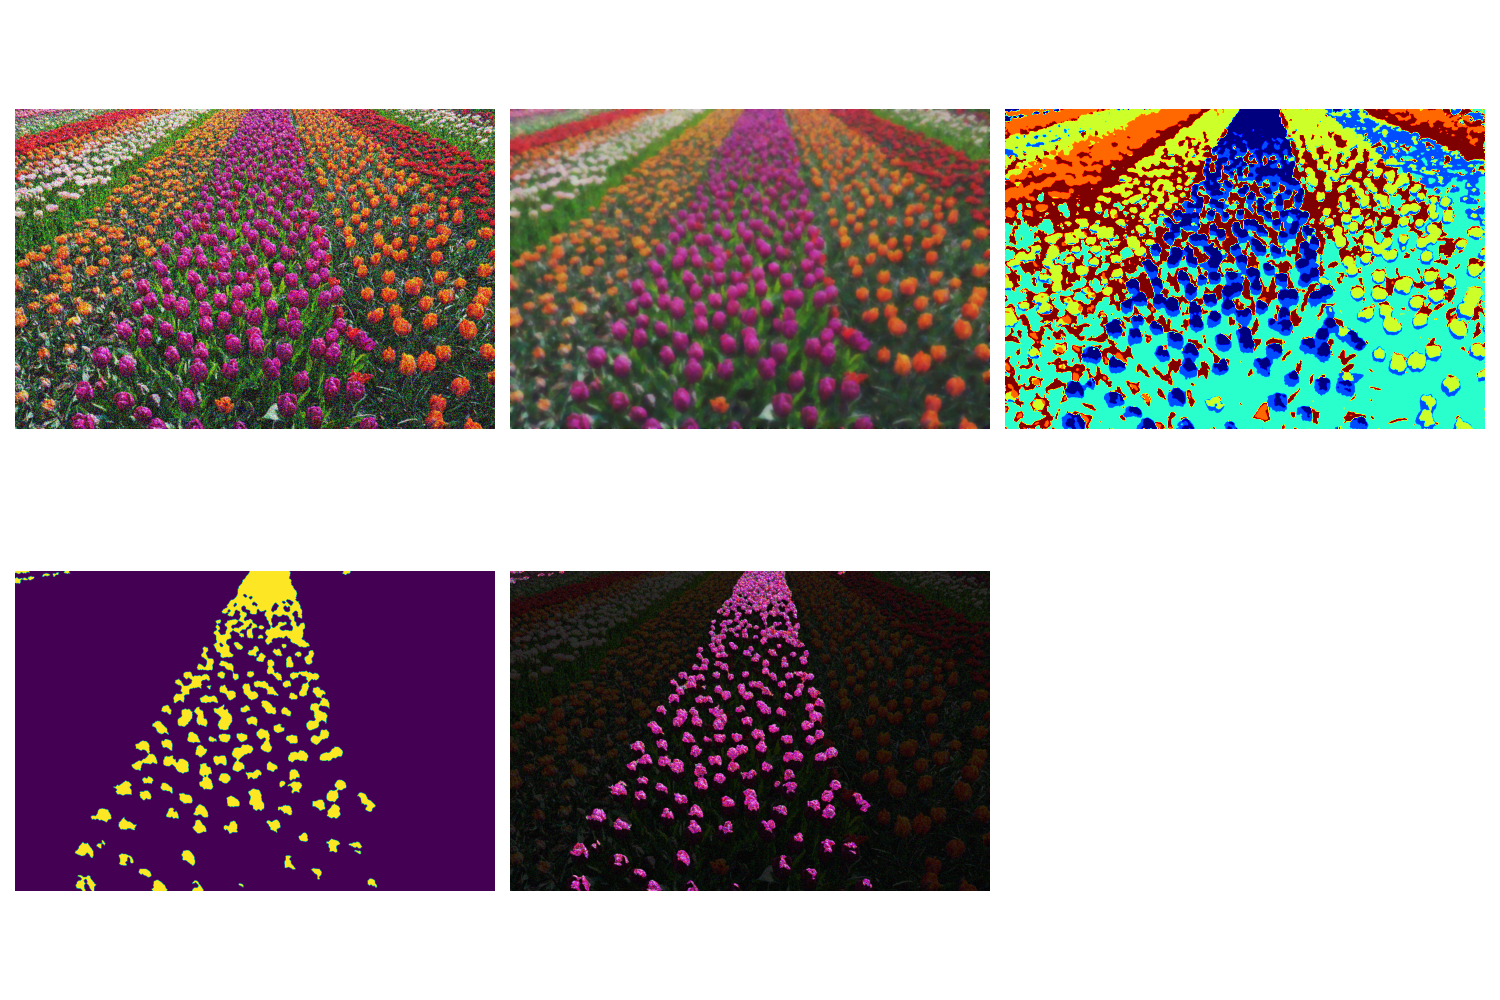
\includegraphics[scale=0.35]{figures/flowers_segmentation.png}
    \caption{Steps of Flowers Segmentation}
    \label{fig:flowers}
\end{figure}

For the flowers image, a more sophisticated segmentation was required in order to handle the three colour channels of the pixels,
as well as to produce a more complex segmentation mask composed of lots of small disconnected regions.
Since the desired segmentation was to be based on the colours present in the image,
it was less important to incorporate local pixel information into the image,
therefore making clustering an appropriate strategy.
In particular, KMeans was chosen, since this method was simple to implement,
commonly used for image segmentation,
and enabled a fixed number of clusters to be specified.
In this case, six clusters was decided as a meaningful number,
corresponding roughly to two shades of green (grass) and four flower colours.
KMeans was implemented as a \texttt{class} in the \texttt{ml} module according to Lloyd's Algorithm \cite{lloyd},
using the kmeans++ \cite{kmeanspp} centroid initialisation method.

Based on this choice of algorithm, Total Variation denoising was used to pre-process the image.
This meant that in the pre-processed image, pixel values were coerced to be similar to those nearby.
This ensured that the clustering algorithm was more stable (since it artificially made the cluster structure of the data more pronounced),
and that the segmentation masks weren't too fine-grained.

The same morphological post-processing from the CT image was used again,
in order to remove segmentation masks that were smaller than the flower buds.

\subsection{Coins Image}

A strong degree of preprocessing was helpful for this image, to assist the segmentation algorithm.
Firstly, the image has been corrupted with vertical columns of pixels that have been masked with zero values.
This was addressed by applying a local median filter.
The locality of this filter was set to each pixel plus its 6 closest horizontal neighbours.
This was wide enough to ensure that in most cases the majority of these 7 pixels are not corrupted,
even in regions where the image is affected more strongly.
An unsharp filter is then used to increase the difference in pixel values within the coin regions compared to just outside of these regions.

To segment all of the coins, the Chan-Vese \cite{chanvese} segmentation algorithm was used.
This method relies on the iterative minimisation of an energy function,
which describes the desired segmentation properties mathematically.
In particular, this technique models the segmentation mask as the set ${x\in\Omega:\phi(x)>0}$,
where $\Omega\subset\mathbb{R}^2$ is the space representing the image,
and $\phi:\Omega\rightarrow[0,1]$ is a function which evolves over the course of the computation.
The function is evolved iteratively to minimise the objective

\begin{align*}
    F(\phi, c_1, c_2) = & \mu\int_{\Omega}\delta(\phi)|\nabla\phi|dxdy + \nu\int_{\Omega}H(\phi)dxdy \\
                    & + \lambda_1\int_{\Omega}|u_0-c_1|^2H(\phi)dxdy + \lambda_2\int_{\Omega}|u_0-c_2|^2(1-H(\phi))dxdy \\
\end{align*}

where $\mu,\nu,\lambda_1,\lambda_2$ are all fixed hyperparameters.
The first two terms serve to regularise the segmentation,
by minimising the length of the segmentation boundary and the segmented area respectively (the area term is ignored in the code).
The second two terms seek to minimise the deviations of pixel values within, and outside, the segmented area from two distinct `representative values',
$c_1$ and $c_2$.
It is worth noting that for any $\phi$, these values minimise the energy when they are the average pixel values in the two corresponding areas of the image.

The algorithm highlighted the background of the image.
Thus to get masks of the coins, the segmentation values were permuted in ${0,1}$ and the segmentation was again post-processed with a morphological closing operation.
The masks were then labelled, and the correct labels were identified via `test pixels', which are seen marking the original image (top-left) in yellow in Figure \ref{fig:coins}

\begin{figure}[hp]
    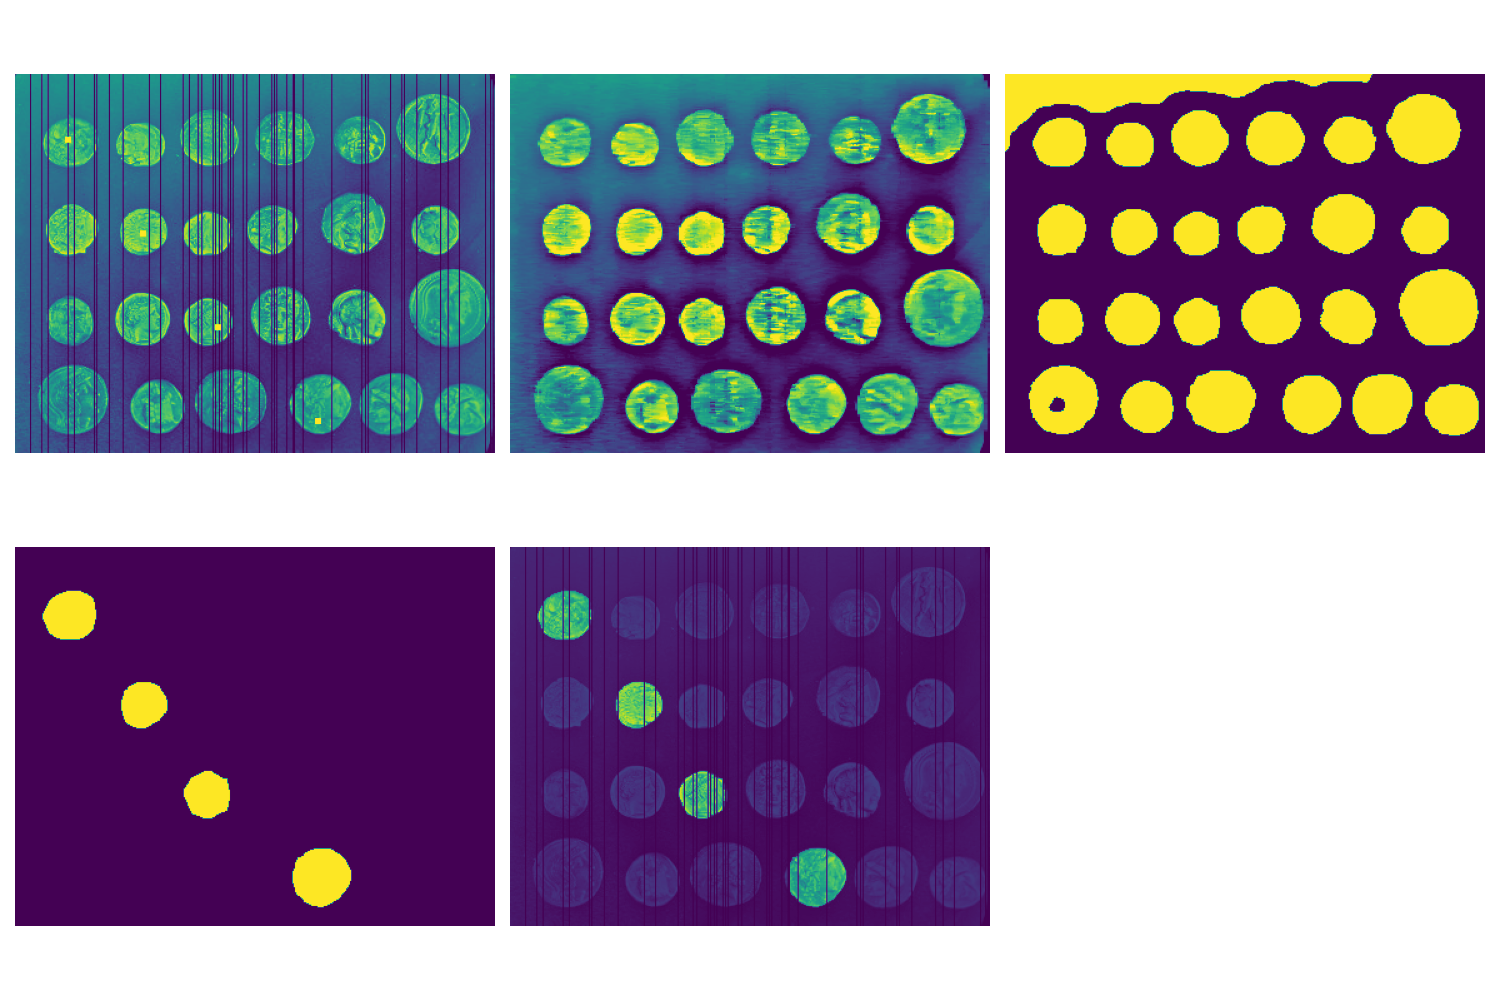
\includegraphics[scale=0.35]{figures/coins_segmentation.png}
    \caption{Steps of Coins Segmentation}
    \label{fig:coins}
\end{figure}

\section{Exploiting Sparsity in Signal Processing}

\subsection{Regression \& Outliers}

\begin{figure}[hp]
    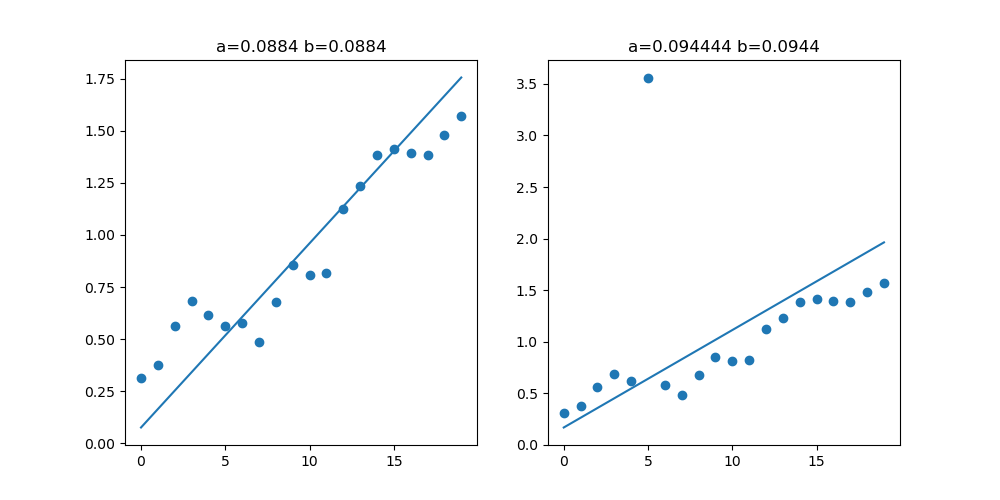
\includegraphics[scale=0.5]{figures/regression_l2.png}
    \caption{L2 Regression}
    \label{fig:regression_l2}
\end{figure}

For simple linear regression problems, the ordinary least squares approach for finding the coefficients is the most ubiquitous.
This is a well-posed optimisation problem that has an analytic solution, and also corresponds to a set of reasonable statistical assumptions in practical scenarios.
This is due to the objective loss function being differentiable and strictly convex; indeed,
\[\text{minimise } \sum_{i=1}^{n}{(ax_i+b-y_i)^2} \quad \text{subject to } (a, b)\in\mathbb{R}^2\]
is therefore solved exactly by finding the unique argument for which the objectives gradient is zero,
\[a^*=\frac{\sum x_i y_i}{\sum x_i^2},\quad b^*=\bar{y} - a^*\bar{x}\]

The original data and L2 regression models are plotted in Figure \ref{fig:regression_l2}.
Comparing the two models, we can see evidence that the least squares coefficients are quite sensitive to outliers.
In the second regression (where the data has the outlier) the coefficients change quite a lot,
so much that this model doesn't appear to fit the main body of data nearly as well as the first model,
even though only one outlier is present.

Using an L1 loss, under the so-called `Least Absolute Deviations (LAD)' model,
is designed to mitigate this sensitivity to outliers.
In both methods, the loss is the sum of some function of the residuals, the quantities $\hat{y_i} - y_i$ where $\hat{y_i}$ denotes the $i^{th}$ model prediction.
However, least squares regression uses the square of these residuals, and so the largest residuals contribute more to the loss,
and therefore more the solution as a result.
By replacing the squared residuals with the absolute residuals in LAD regression, all residuals contribute equally,
which means that the optimal LAD coefficients should be less sensitive to the presence of a few outliers.
On the other hand, the LAD regression framework is much more pathological.
The objective function is not differentiable, nor is it strictly convex, meaning that solutions are not guaranteed to be unique.
There is no analytic formula for any of the solutions.
In light of these issues, the Subgradient Method was used to find the L1 coefficients.

The Subgradient Method is similar to usual gradient descent, but extended to non-differentiable functions such as the L1 regression objective,
\[L(a,b) = \sum_{i=1}^{n}{|ax_i + b - y_i|}\]

We must replace the usual gradient term for the step direction with a non-unique `subgradient', a function $g:\mathbb{R}^2\rightarrow\mathbb{R}^2$ satisfying
\[f(x')\geq f(x) + g(x)^T(x'-x) \quad \forall x, x' \in\mathbb{R}^2\]

All convex functions such as the L1 objective permit at least a subgradient if not a true derivative \cite{convex},
and indeed the subgradient is only non-unique at points where the function is non-differentiable.
The subgradient chosen was based on a choice of subgradient for the function $z\rightarrow|z|$,
namely

\[
\text{sgn}(x) =
\begin{cases}
    1,   &\quad\text{if }x>0,\\
    -1,  &\quad\text{if }x<0,\\
    0,   &\quad\text{otherwise.}\\
\end{cases}
\]

which in turn gave the subgradient

\[(x^T\text{sgn}(ax+b-y), \text{sgn}(ax+b-y))\]

where $\text{sgn}$ is applied elementwise.
The results of the Subgradient Method regression are shown in Figure \ref{fig:regression_l1}.
We see that this method is much more robust against outliers, with similar coefficients found in both cases.
In addition, the coefficients found for the non-outlier case are fairly similar to the least squares coefficients.
The downsides of this method are that the coefficients are somewhat sensitive to the choice of learning rate and initial coefficient.

\begin{figure}[hp]
    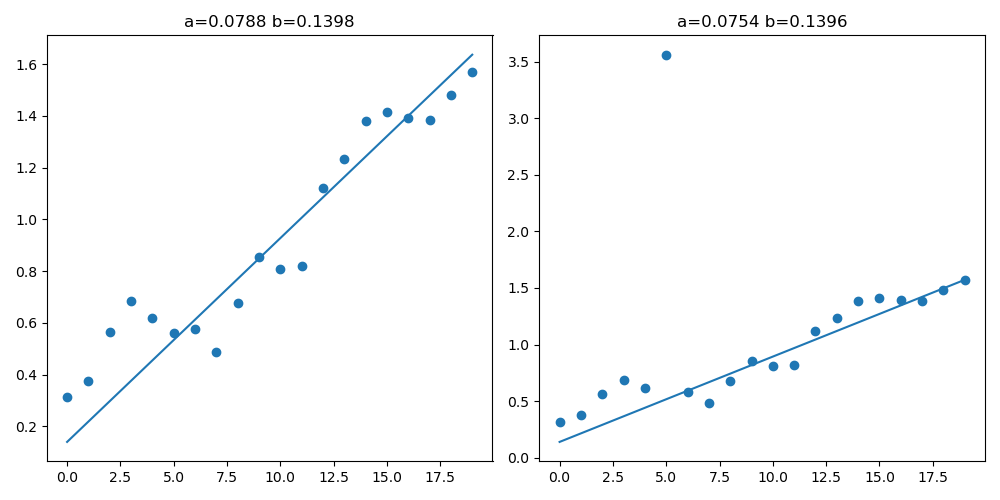
\includegraphics[scale=0.5]{figures/regression_l1.png}
    \caption{L1 Regression}
    \label{fig:regression_l1}
\end{figure}

\subsection{Undersampling}

In this part we reconstruct a sparse signal from two different samples of its transformation into k-space.
We create a vector with only 10\% non-zero entries and then add a small amount of Gaussian noise to simulate a sparse signal.
We then Fourier transform this and take two 4-fold undersampling strategies:
\begin{itemize}
    \item equidistant sampling; where every fourth entry in k-space is sampled (though the offset is randomly chosen), and,
    \item random sampling; where exactly one quarter of the entries are sampled, each entry having equal selection probability.
\end{itemize}
In both cases, the non-sampled entries in k-space are masked with zeros.

\begin{figure}[hp]
    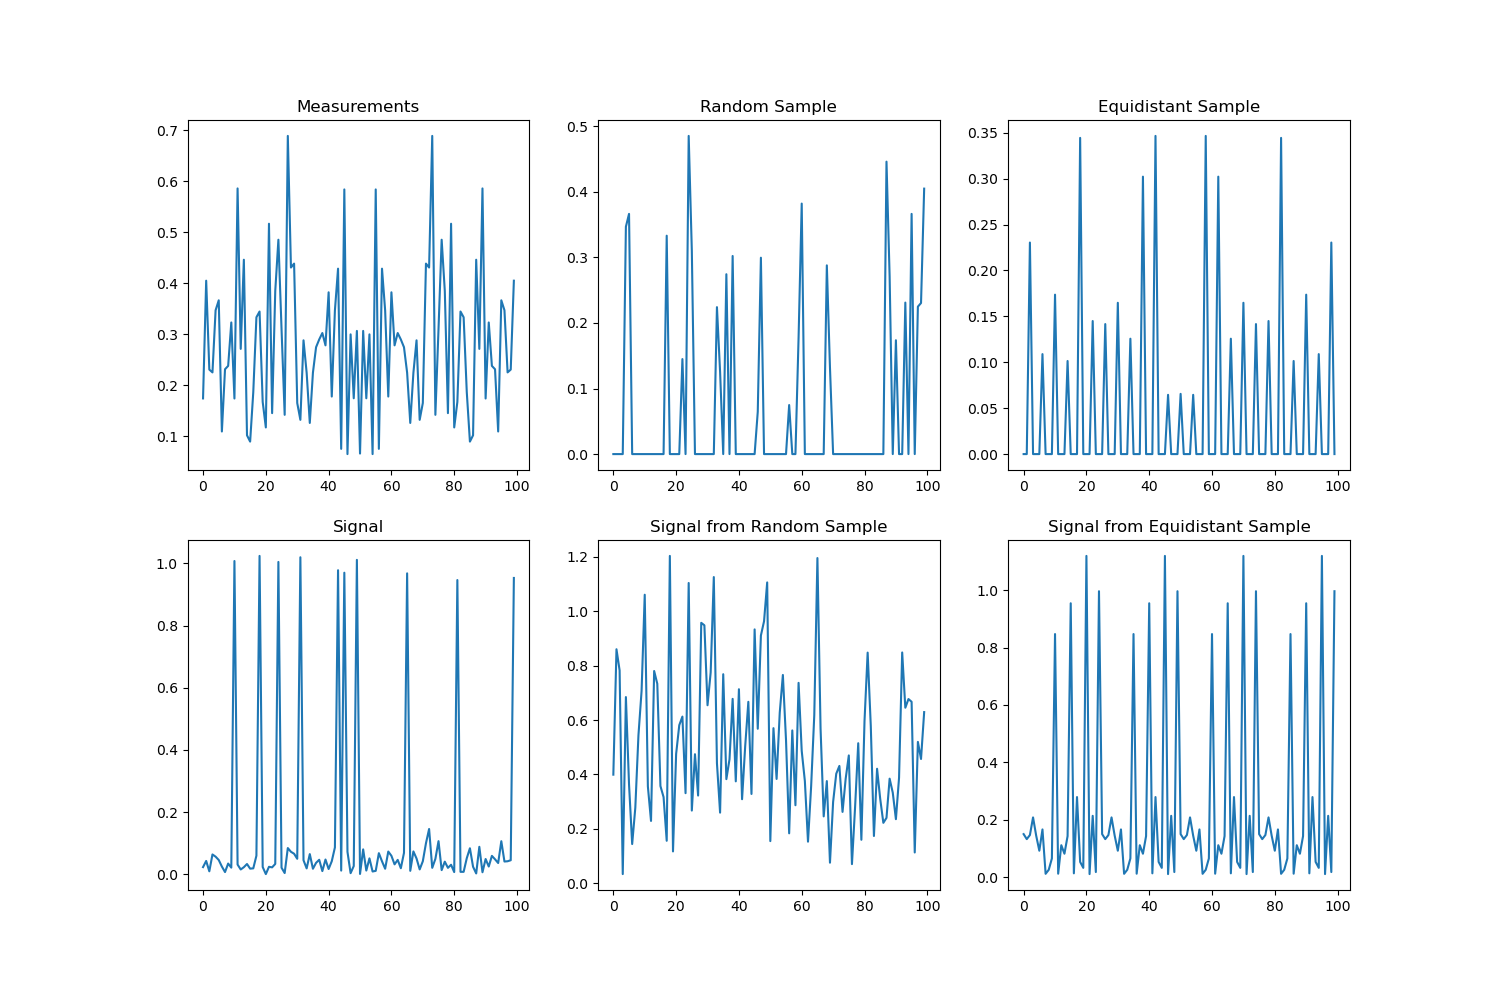
\includegraphics[scale=0.36]{figures/signal.png}
    \caption{Signals and measurements}
    \label{fig:signal}
\end{figure}

The samples simulate measurements ($y$) taken in a real-life scenario, which are some function of the true underlying signal ($x$),
in this case the signal's Fourier Transform.
In both cases the samples were used to reconstruct the signal via Iterative Soft Thresholding,
which in this case involved repeating the following steps
\begin{itemize}
    \item transforming to the signal domain (inverse Fourier transform),
    \item soft-thresholding the approximate signal,
    \item transforming back to the measurement domain (Fourier transform), and,
    \item enforcing data consistency; only zero-filled measurements from the original sample are allowed to be altered.
\end{itemize}

In Figure \ref{fig:signal_reconstruct} we see the results of this reconstruction using 100 iterations and $\lambda=0.02$ for the soft-thresholding.
Importantly, the algorithm only had an effect on the signal that was inferred from the random sample of measurements.
In this case, the algorithm improved the accuracy of the signal reconstruction,
as shown by the L2 distance of the reconstructed measurements compared to the true measurements decreasing over time.

This case study serves as a demonstration of the power of Compressed Sensing,
when done correctly.
Compressed Sensing emerged in the signal processing literature in the mid 2000s,
offering a radically efficient way of acquiring signals using far fewer measurements than suggested by classical results in the field.
The well-established Nyquist-Shannon sampling theorem suggests that the sampling rate should be more than twice the greatest frequency present in the true data,
as this ensures perfect reconstruction according to the result \cite{shannon}.
However, this sampling rate is notably framed as a sufficient, rather than necessary condition in the theorem,
and Compressed Sensing develops a framework in which under certain assumptions,
an excellent signal reconstruction can occur with a much more economical sampling scheme.
In particular, we must assume:
\begin{enumerate}
    \item incoherence; this is achieved in general by a `random' subsampling scheme, and,
    \item sparsity; the measurements must have a sparse representation in some transformed domain, such as Fourier or wavelet decomposition.
\end{enumerate}

By undersampling by a factor of 4 we generate a highly underdetermined inverse problem,
namely that infintely many signals $x$ can be mapped to the measurements $y$ by the Fourier transform and 4-fold undersampling.
Heuristically, the assumption of sparsity of $x$ `narrows down' this pool of candidate signals,
leading to an accurate (though imperfect) reconstruction of the signal in the random sampling scheme.
The equidistant sampling scheme violates the first assumption of incoherence,
leading to a reconstruction which cannot be improved.
This scheme leads to the `aliasing' effect that the Nyquist-Shannon sampling theorem was designed to mitigate against.
Namely, by undersampling in this way, high frequency components in the data are confounded with low frequency components,
consituting an irreversible loss of information.

\begin{figure}[hp]
    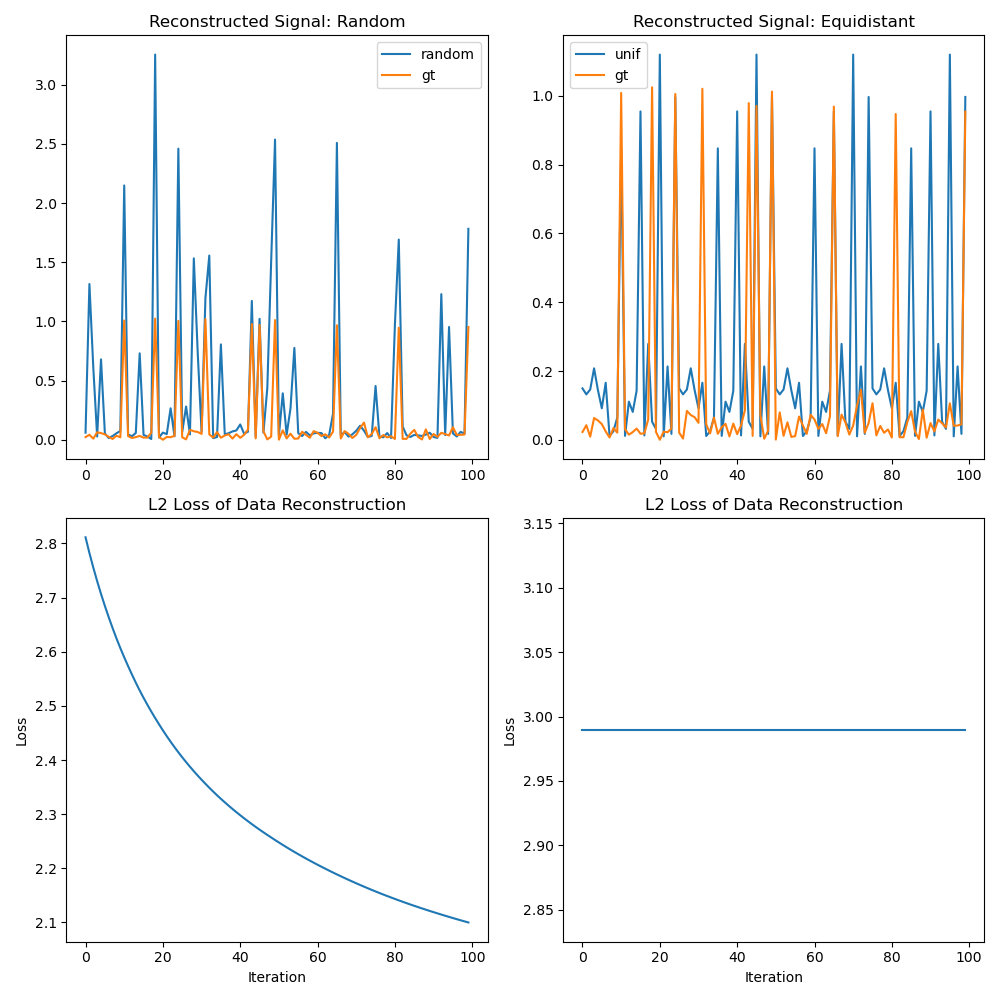
\includegraphics[scale=0.5]{figures/signal_reconstruct.png}
    \caption{Iterative Soft Thresholding Reconstructions}
    \label{fig:signal_reconstruct}
\end{figure}

\subsection{Wavelet Decomposition}

In this part, we explore the relevance of sparsity to image processing.
Figure \ref{fig:river_img} (left) shows an image which was passed through a Daubechies wavelet transform.
The two other images show the effects of reconstructing this image by directly applying the inverse wavelet transform.
The reconstruction is almost identical to the original, achieving a Structural Similarity Index which is perfect to two decimal places.
Crucially, the right-most image in Figure \ref{fig:river_img} shows that where there are pixel value errors,
they are greatest in the main central part of the image (where this plot is brighter on average).
The errors are generally smaller in the empty space around the image, although there is an unusual periodic pattern of errors here.

\begin{figure}[hp]
    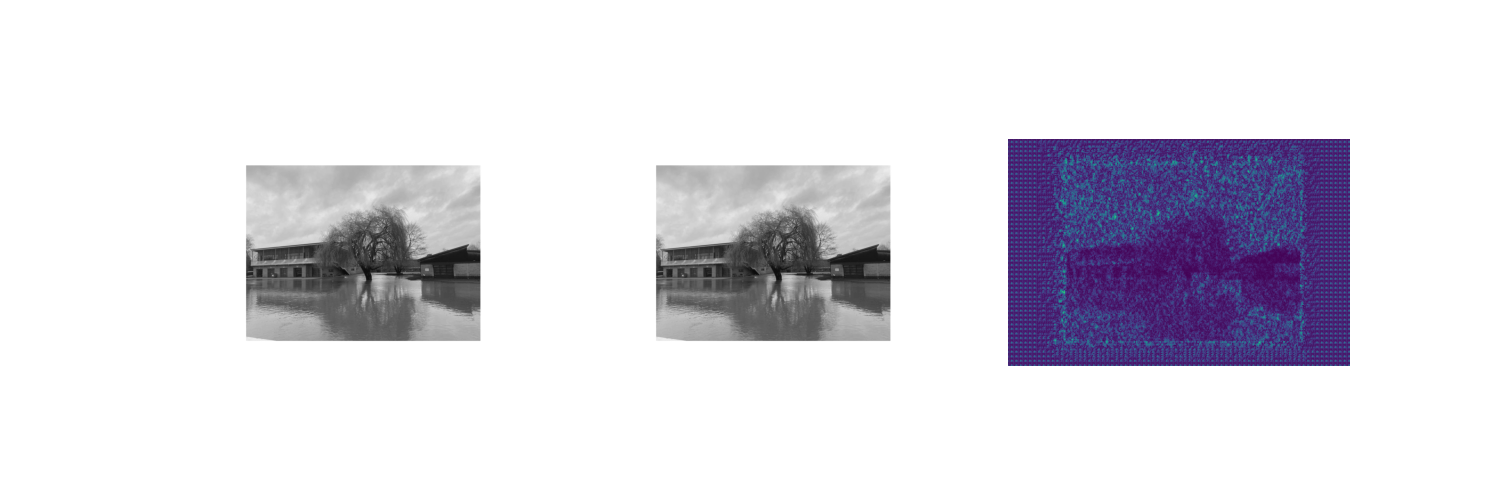
\includegraphics[scale=0.35]{figures/river_img.png}
    \caption{River Image and Reconstruction from Wavelet Decomposition}
    \label{fig:river_img}
\end{figure}

Figure \ref{fig:wavelet_transform} shows the wavelet transform of the river image.
On the left we see the original coefficients \footnote{clipped in the 0.5-99.5\% range to improve visibility},
while the right hand side indicates which of these lie in the top 15\% of coefficients.
We see that even removing 85\% of the expressive range of the coefficients in the wavelet domain,
the representation still encodes meaningful features relating to the image - this is a sparse representation of the image.

\begin{figure}[hp]
    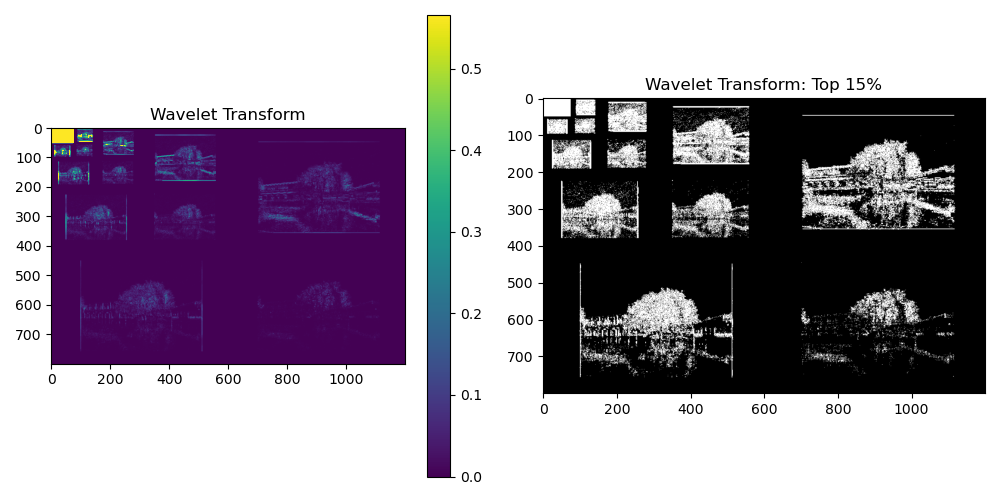
\includegraphics[scale=0.5]{figures/wavelet_transform.png}
    \caption{River Image and Reconstruction from Wavelet Decomposition}
    \label{fig:wavelet_transform}
\end{figure}

As a result, clipping coefficients whose absolute value is below this threshold and then performing the inverse transform will



\section{Algorithms for Solving Inverse Problems}
\subsection{Convergence of Gradient Descent}

Gradient Descent.

We can prove that the given function $f:\mathbb{R}^2\rightarrow\mathbb{R}$ defined

\[f(x_1,x_2) = x_1^2 + \frac{x_2^2}{2}\]

is $L$-smooth with $L=2$ via the following

The result given is, for learning rate $\eta=\frac{1}{L}$, and an $L$-smooth function $f$,

\[f(x_K) - f(x^*) \leq \frac{L||x_0-x^*||_2^2}{2K}\]

It is important to note that this is an estimate that gives the accuracy as $\mathcal{O}(\frac{1}{K})$.
We can use it to compute the estimate the number of steps to required to reach $\epsilon=0.01$,
but this will be an upper bound.
Nonetheless, we can set the right-hand side to $\epsilon$ and rearrange to give:

\[K = \frac{L||x_0-x^*||_2^2}{2\epsilon}\]

Substituting $\epsilon=0.01$, $x^*=(0,0)$, $x_0=(1,1)$, $L=2$, we get $K=200$.



\subsection{LGD}



\bibliographystyle{IEEEtran}
\bibliography{Biblio}

\appendix

\section{Statement on the use of auto-generation tools}

\end{document}
